\documentclass{beamer}
\usepackage{../../shared/styles/custom}


%\beamerdefaultoverlayspecification{<+->}


	\ifx\relax#1\relax  \item \else \item[#1] \fi
	\abovedisplayskip=0pt\abovedisplayshortskip=0pt~\vspace*{-\baselineskip}}




\title{Naive Bayes}
\date{\today}
\author{Nipun Batra}
\institute{IIT Gandhinagar}
\begin{document}
  \maketitle
  
  
  
% \section{Linear Regression}

\begin{frame}{Bayesian Networks}
    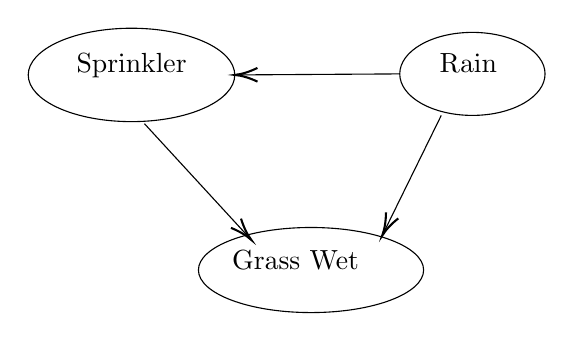
\begin{tikzpicture}[x=0.75pt,y=0.75pt,yscale=-1,xscale=1]
        %uncomment if require: \path (0,300); %set diagram left start at 0, and has height of 300
        
        %Shape: Ellipse [id:dp7372359450600154] 
        \draw   (100,142.5) .. controls (100,130.07) and (122.27,120) .. (149.75,120) .. controls (177.23,120) and (199.5,130.07) .. (199.5,142.5) .. controls (199.5,154.93) and (177.23,165) .. (149.75,165) .. controls (122.27,165) and (100,154.93) .. (100,142.5) -- cycle ;
        %Shape: Ellipse [id:dp773307115438193] 
        \draw   (279,142) .. controls (279,130.95) and (294.67,122) .. (314,122) .. controls (333.33,122) and (349,130.95) .. (349,142) .. controls (349,153.05) and (333.33,162) .. (314,162) .. controls (294.67,162) and (279,153.05) .. (279,142) -- cycle ;
        %Straight Lines [id:da30385042687371255] 
        \draw    (279,142) -- (201.5,142.49) ;
        \draw [shift={(199.5,142.5)}, rotate = 359.64] [color={rgb, 255:red, 0; green, 0; blue, 0 }  ][line width=0.75]    (10.93,-3.29) .. controls (6.95,-1.4) and (3.31,-0.3) .. (0,0) .. controls (3.31,0.3) and (6.95,1.4) .. (10.93,3.29)   ;
        %Shape: Ellipse [id:dp08595332977182091] 
        \draw   (182,236.5) .. controls (182,225.18) and (206.29,216) .. (236.25,216) .. controls (266.21,216) and (290.5,225.18) .. (290.5,236.5) .. controls (290.5,247.82) and (266.21,257) .. (236.25,257) .. controls (206.29,257) and (182,247.82) .. (182,236.5) -- cycle ;
        %Straight Lines [id:da6920360079941172] 
        \draw    (299,162) -- (271.38,218.2) ;
        \draw [shift={(270.5,220)}, rotate = 296.17] [color={rgb, 255:red, 0; green, 0; blue, 0 }  ][line width=0.75]    (10.93,-3.29) .. controls (6.95,-1.4) and (3.31,-0.3) .. (0,0) .. controls (3.31,0.3) and (6.95,1.4) .. (10.93,3.29)   ;
        %Straight Lines [id:da8073837163630633] 
        \draw    (156,166) -- (206.15,220.53) ;
        \draw [shift={(207.5,222)}, rotate = 227.4] [color={rgb, 255:red, 0; green, 0; blue, 0 }  ][line width=0.75]    (10.93,-3.29) .. controls (6.95,-1.4) and (3.31,-0.3) .. (0,0) .. controls (3.31,0.3) and (6.95,1.4) .. (10.93,3.29)   ;
        
        % Text Node
        \draw (122,131) node [anchor=north west][inner sep=0.75pt]   [align=left] {Sprinkler};
        % Text Node
        \draw (297,131) node [anchor=north west][inner sep=0.75pt]   [align=left] {Rain};
        % Text Node
        \draw (197,226) node [anchor=north west][inner sep=0.75pt]   [align=left] {Grass Wet};
        
        
        \end{tikzpicture}
        
\begin{itemize}
	
	
	\item Nodes are random variables.
	\item Edges denote direct impact

	
\end{itemize}
\end{frame}

\begin{frame}{Example}
\begin{itemize}

\item Grass can be wet due to multiple reasons:
\begin{itemize}
    \item Rain
    \item Sprinkler
\end{itemize}
\item Also, if it rains, then sprinkler need not be used.
\end{itemize}

    


	

\end{frame}

\begin{frame}{Bayesian Nets}
    $P(X_{1},X_{2},X_{3},\dots,X_{N})$ denotes the joint probability, where $X_{i}$ are random variables.
    \begin{equation*}
        P(X_{1},X_{2},X_{3},\dots,X_{N}) = \Pi_{k=1}^{N} P(X_{k} | parents(X_{k}))
    \end{equation*}
    
    
    \begin{equation*}
        P(S,G,R) =  P(G|S,R)P(S|R)P(R)
    \end{equation*}
    
\end{frame}


\begin{frame}{Spam Email Classification}
    \begin{itemize}[<+->]
        \item $y \in\{0,1\}$ where 0 means not spam and 1 means spam
        \item From the emails construct a vector $X$.
        \item $\left[\begin{array}{c}a \\ a n \\ \vdots \\ \text { computer } \\ \vdots \\ \text { lotery } \\ \vdots \\ 200\end{array}\right]\}$ N words
        \item The vector has ones if the word is present, and zeros is the word is absent.
        \item Each email corresponds to vector/feature of length N containing zeros or ones.
    \end{itemize}
     
\end{frame}

\begin{frame}{Naive Bayes}
    \begin{itemize}[<+->]
        \item Classification model
        \item Scalable
        \item Generative and Bayesian
        \item Usually a simple/good baselines
        \item  We want to model $P(class (y) \mid$ features (x)) 
        \item We can use Bayes rule as follows:
        $P(class(y) \mid \text { features (x) })=\frac{P(\text { features (x) } \mid class(y)) P(class(y))}{P(\text { features (x) })}$
    \end{itemize}
    
   

\end{frame}

\begin{frame}{Quick Question}
    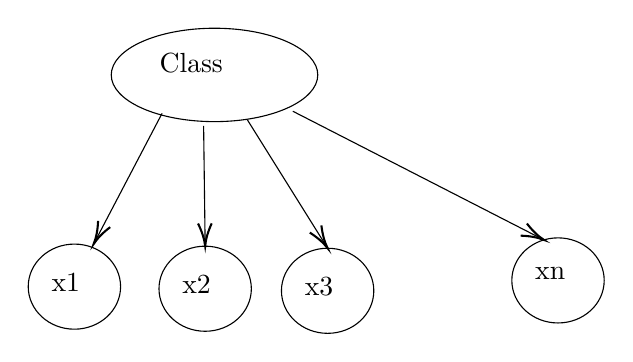
\begin{tikzpicture}[x=0.75pt,y=0.75pt,yscale=-1,xscale=1]
        %uncomment if require: \path (0,300); %set diagram left start at 0, and has height of 300
        
        %Shape: Ellipse [id:dp7372359450600154] 
        \draw   (100,142.5) .. controls (100,130.07) and (122.27,120) .. (149.75,120) .. controls (177.23,120) and (199.5,130.07) .. (199.5,142.5) .. controls (199.5,154.93) and (177.23,165) .. (149.75,165) .. controls (122.27,165) and (100,154.93) .. (100,142.5) -- cycle ;
        %Shape: Ellipse [id:dp08595332977182091] 
        \draw   (60,244.5) .. controls (60,233.18) and (69.96,224) .. (82.25,224) .. controls (94.54,224) and (104.5,233.18) .. (104.5,244.5) .. controls (104.5,255.82) and (94.54,265) .. (82.25,265) .. controls (69.96,265) and (60,255.82) .. (60,244.5) -- cycle ;
        %Straight Lines [id:da8073837163630633] 
        \draw    (124.5,161) -- (92.43,222.23) ;
        \draw [shift={(91.5,224)}, rotate = 297.65] [color={rgb, 255:red, 0; green, 0; blue, 0 }  ][line width=0.75]    (10.93,-3.29) .. controls (6.95,-1.4) and (3.31,-0.3) .. (0,0) .. controls (3.31,0.3) and (6.95,1.4) .. (10.93,3.29)   ;
        %Shape: Ellipse [id:dp023537100462790228] 
        \draw   (123,245.5) .. controls (123,234.18) and (132.96,225) .. (145.25,225) .. controls (157.54,225) and (167.5,234.18) .. (167.5,245.5) .. controls (167.5,256.82) and (157.54,266) .. (145.25,266) .. controls (132.96,266) and (123,256.82) .. (123,245.5) -- cycle ;
        %Shape: Ellipse [id:dp4079980413843134] 
        \draw   (182,246.5) .. controls (182,235.18) and (191.96,226) .. (204.25,226) .. controls (216.54,226) and (226.5,235.18) .. (226.5,246.5) .. controls (226.5,257.82) and (216.54,267) .. (204.25,267) .. controls (191.96,267) and (182,257.82) .. (182,246.5) -- cycle ;
        %Shape: Ellipse [id:dp6596498120094669] 
        \draw   (293,241.5) .. controls (293,230.18) and (302.96,221) .. (315.25,221) .. controls (327.54,221) and (337.5,230.18) .. (337.5,241.5) .. controls (337.5,252.82) and (327.54,262) .. (315.25,262) .. controls (302.96,262) and (293,252.82) .. (293,241.5) -- cycle ;
        %Straight Lines [id:da15595132436398473] 
        \draw    (144.5,167) -- (145.22,223) ;
        \draw [shift={(145.25,225)}, rotate = 269.26] [color={rgb, 255:red, 0; green, 0; blue, 0 }  ][line width=0.75]    (10.93,-3.29) .. controls (6.95,-1.4) and (3.31,-0.3) .. (0,0) .. controls (3.31,0.3) and (6.95,1.4) .. (10.93,3.29)   ;
        %Straight Lines [id:da8789748623945954] 
        \draw    (165.5,164) -- (203.19,224.3) ;
        \draw [shift={(204.25,226)}, rotate = 237.99] [color={rgb, 255:red, 0; green, 0; blue, 0 }  ][line width=0.75]    (10.93,-3.29) .. controls (6.95,-1.4) and (3.31,-0.3) .. (0,0) .. controls (3.31,0.3) and (6.95,1.4) .. (10.93,3.29)   ;
        %Straight Lines [id:da7453498794319566] 
        \draw    (187.5,160) -- (306.72,221.09) ;
        \draw [shift={(308.5,222)}, rotate = 207.13] [color={rgb, 255:red, 0; green, 0; blue, 0 }  ][line width=0.75]    (10.93,-3.29) .. controls (6.95,-1.4) and (3.31,-0.3) .. (0,0) .. controls (3.31,0.3) and (6.95,1.4) .. (10.93,3.29)   ;
        
        % Text Node
        \draw (122,131) node [anchor=north west][inner sep=0.75pt]   [align=left] {Class};
        % Text Node
        \draw (70,237) node [anchor=north west][inner sep=0.75pt]   [align=left] {x1};
        % Text Node
        \draw (133,238) node [anchor=north west][inner sep=0.75pt]   [align=left] {x2};
        % Text Node
        \draw (192,239) node [anchor=north west][inner sep=0.75pt]   [align=left] {x3};
        % Text Node
        \draw (303,234) node [anchor=north west][inner sep=0.75pt]   [align=left] {xn};
        
        
        \end{tikzpicture}
    
    
    \pause \begin{equation*}
        P(x_{1},x_{2},x_{3},\dots,x_{N} \vert y) = P(x_{1}|y) P(x_{2}|y) \dots P(x_{N}|y)
    \end{equation*}
    \pause Why is Naive Bayes model called Naive? \\

    \pause Naive assumption $x_{i}$ and $x_{i+1}$ are independent given y
    \[
    \text { i.e. }  p\left(x_{2} \mid x_{1}, y\right)=p\left(x_{2} \mid y\right)
    \]

\end{frame}


\begin{frame}{Frame Title}
    It assumes that the features are independent during modelling, which is generally not the case.
\end{frame}

\begin{frame}{What do we need to predict?}
    \begin{equation*}
        P(y|x_{1},x_{2},\dots,x_{N}) =  \frac{P(x_{1},x_{2},\dots,x_{N}|y)P(y)}{P(x_{1},x_{2},\dots,x_{N})}
    \end{equation*}
\end{frame}


\begin{frame}{Spam Mail Classification}
    Probability of $x_{i}$ being a spam email\\
    $$
    P(x_{i} = 1|y = 1) = \frac{\text{Count} (x_{i} = 1 \text{ and } y = 1)}{\text{Count }(y=1)}
    $$
    
    Similarly,
    
    $$
    P(x_{i} = 0|y = 1) = \frac{\text{Count} (x_{i} = 0 \text{ and } y = 1)}{\text{Count }(y=1)}
    $$
    
    
\end{frame}


\begin{frame}{Spam Mail classification}
    $$
        P(y = 1) = \frac{\text{Count }(y=1) }{\text{Count }(y=1) +\text{Count }(y=0) }
    $$
    
    Similarly,
    
    $$
        P(y = 0) = \frac{\text{Count }(y=0) }{\text{Count }(y=1) +\text{Count }(y=0) }
    $$
    
    
    
\end{frame}

\begin{frame}{Example}
    lets assume that dictionary is $[w_{1},w_{2},w_{3}]$
    
    
    \begin{tabular}{c|c|c|c|c}
    Index&$w_{1}$&$w_{2}$&$w_{3}$&y\\
    \hline
    \hline
         1 & 0 & 0 & 0 & 1  \\
         2 & 0 & 0 & 0 & 0  \\
         3 & 0 & 0 & 0 & 1  \\
         4 & 1 & 0 & 0 & 0  \\
         5 & 1 & 0 & 1 & 1  \\
         6 & 1 & 1 & 1 & 0  \\
         7 & 1 & 1 & 1 & 1  \\
         8 & 1 & 1 & 0 & 0  \\
         9 & 0 & 1 & 1 & 0  \\
         10 & 0 & 1 & 1 & 1  \\
    \end{tabular}
\end{frame}

\begin{frame}{Spam Classification}
    if y=0
    \begin{itemize}
        \item $P(w_{1}=0\vert y=0)$ = $\frac{3}{5}$ = 0.6 \\
        \item $P(w_{2}=0\vert y=0)$ = $\frac{2}{5}$ = 0.4 \\
        \item $P(w_{3}=0\vert y=0)$ = $\frac{3}{5}$ = 0.6 \\
    \end{itemize}
    P(y=0) = 0.5\\
    Similarly, if y=1
    \begin{itemize}
        \item $P(w_{1}=1\vert y=1)$ = $\frac{2}{5}$ = 0.4 \\
        \item $P(w_{2}=1\vert y=1)$ = $\frac{1}{5}$ = 0.2 \\
        \item $P(w_{3}=1\vert y=1)$ = $\frac{3}{5}$ = 0.6 \\
    \end{itemize}
    P(y=1) = 0.5
\end{frame}

\begin{frame}{Spam Classification}
    
    Given, test email {0,0,1}, classify using naive bayes
    \pause 
$$
        P(y=1\vert w_{1}=0,w_{2} = 0,w_{3}=1) 
$$
$$ = \frac{P(w_{1}=0|y=1) P(w_{2}=0|y=1) P(w_{3}=1|y=1) P(y=1)}{P(w_{1}=0, w_{2}=0, w_{3}=1)}
    $$
    $$ = \frac{0.6\times 0.8 \times 0.6 \times 0.5}{Z}
    $$
    
\pause Similarly, we can calculate $P(y=0\vert w_{1}=0,w_{2} = 0,w_{3}=1) = \frac{0.6*0.4*0.6*0.5}{Z} $

\pause $\frac{P\left(y=1 \mid w_{1}=0, w_{2}=0, w_{3}=1\right)}{P\left(y=0 \mid w_{1}=0, w_{2}=0, w_{3}=1\right)} = 2 > 1$. Thus, classified as a spam example.
    
\end{frame}

\begin{frame}{Naive Bayes for email/sentiment analysis}
    \begin{itemize}
        \item ``This product is pathetic''. We would assume the sentiment of such a sentence to be negative. Why? Presenece of ``pathetic''
        \item Naive bayes would store the probabilities of words belonging to positive or negative sentiment.
        \item Good is positive, Bad is negative
        \item What about: This product is not bad. Naive Bayes is very naive and does not account for sequential aspect of data.
    \end{itemize}
    
\end{frame}

%\begin{frame}{Spam Classification}
%    
%    Calculate, $P(y=1 \vert w_{1}=0, w_{2}=0, w_{3}=1)$ and $P(y=1 \vert w_{1}=0, w_{2}=0, w_{3}=1)$
%    
%    if $P(y=1 \vert w_{1}=0, w_{2}=0, w_{3}=1)$ $\gt$ $P(y=0 \vert w_{1}=0, w_{2}=0, w_{3}=1)$, then it is a spam mail
%\end{frame}


\begin{frame}{Gaussian Naive Bayes}
    Let us generate some normally distributed height data assuming Height (male) $\sim \mathcal{N}(\mu_1 = 6.1, \sigma_1^2 = 0.6)$
 and Height (female) $\sim \mathcal{N}(\mu_2 = 5.3, \sigma_2^2 = 0.9)$
    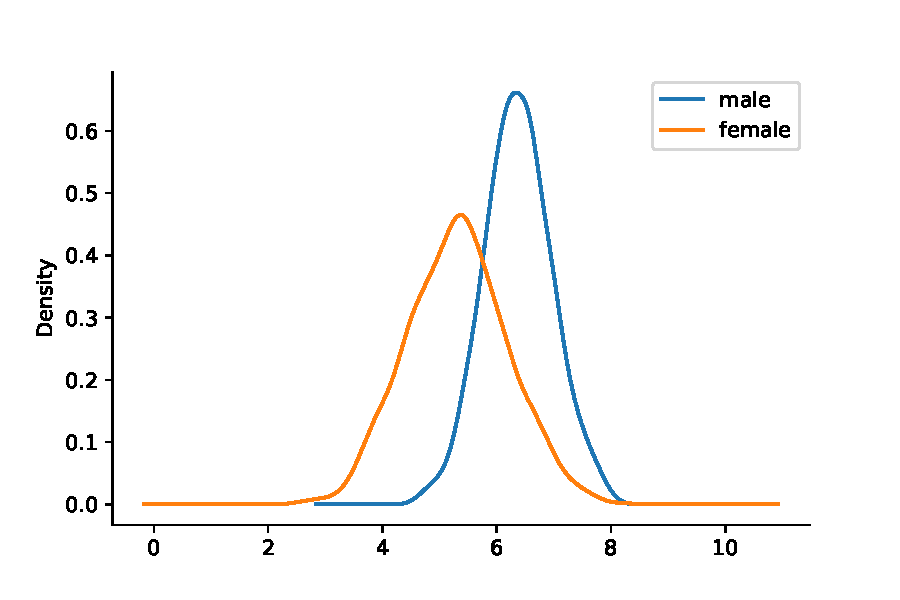
\includegraphics[width=0.9\textwidth]{kde1.pdf}
\end{frame}

\begin{frame}{Gaussian Naive Bayes}
    Let us generate some normally distributed height data assuming Height (male) $\sim \mathcal{N}(\mu_1 = 6.1, \sigma_1^2 = 0.6)$
 and Height (female) $\sim \mathcal{N}(\mu_2 = 5.3, \sigma_2^2 = 0.9)$
    \includegraphics[width=0.9\textwidth]{violin.pdf}
\end{frame}

\begin{frame}{Gaussian Naive Bayes}
    Would you expect a person to height 5.5 as a female or male? And why? 

    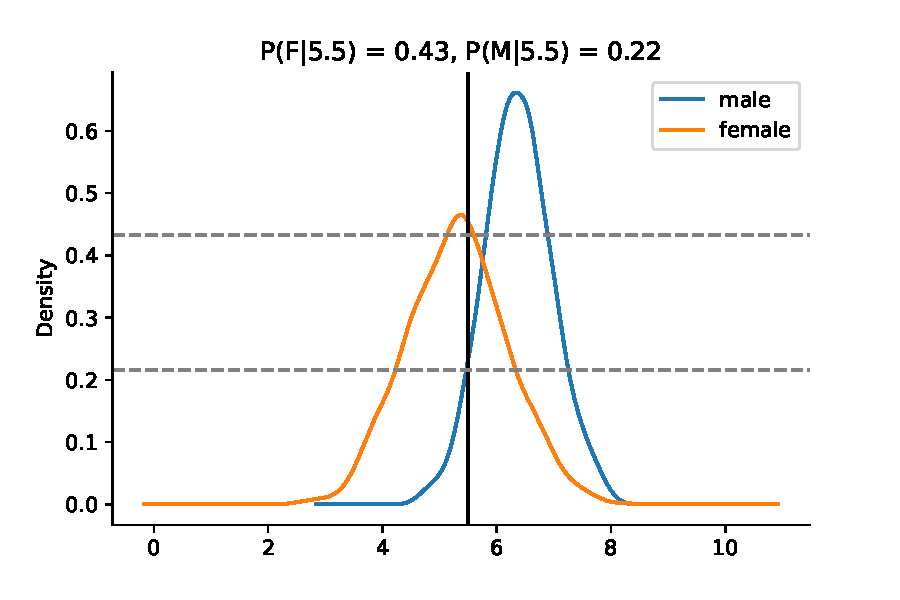
\includegraphics[width=0.9\textwidth]{kde2.pdf}
\end{frame}

\begin{frame}{Gaussian Naive Bayes}
    We have classes $C_{1}, C_{2}, C_{3},\dots, C_{k}$\\
    There is a continuous attribute x\\
    For Class k 
    \begin{itemize}
        \item $\mu_{k} = Mean(x \vert y(x) = C_{k})$
        \item $\sigma_{k}^{2} = Variance(x \vert y(x)=C_{k})$
    \end{itemize}
    
\end{frame}

\begin{frame}{Guassian Naive Bayes}
    Now for x = some observation 'v'\\
    \begin{equation*}
        P(x=v\vert C_{k}) = \frac{1}{\sqrt{2\pi \sigma_{k}^{2}}} \exp^{\frac{-(v-\mu_{k})^{2}}{2\sigma_{k}^{2}}}
    \end{equation*}
\end{frame}

\begin{frame}{Gaussian Naive Bayes (2d example)}
    Would you expect a person to height 5.5 and weight 80 as a female or male? And why? \\
    \pause Note: no cross covariance! Remember all features are independent.

    \includegraphics[width=0.9\textwidth]{kde2d.pdf}
\end{frame}

\begin{frame}{Wikipedia Example}

    \begin{center}
    \begin{tabular}{|c|c|c|c|}
    \hline
    Height&Weight&Footsize&Gender\\
    \hline
    \hline
         6 & 180& 12& M \\
         5.92 & 190& 11& M \\
         5.58 & 170& 12& M \\
         5.92 & 165& 10& M \\
         5 & 100& 6& F \\
         5.5 & 100& 6& F \\
         5.42 & 130& 7& F \\
         5.75 & 150& 7& F \\
         \hline
    \end{tabular}
    
    \end{center}
    
\end{frame}

\begin{frame}{Example}
    \begin{center}
        
    
    \begin{tabular}{|c|c|c|}
    \hline
     &Male&Female\\
     \hline
     \hline
     Mean (height) & 5.855 & 5.41  \\
     Variance (height) & 3.5 $\times$ $10^{-2}$ & 9.7 $\times$ $10^{-2}$  \\
     Mean (weight) & 176.25 & 132.5  \\
     Variance (weight) & 1.22 $\times$ $10^{2}$ & 5.5 $\times$ $10^{2}$   \\
     Mean (Foot) & 11.25 & 7.5  \\
     Variance (Foot) & 9.7 $\times$ $10^{-1}$ & 1.67  \\
    \hline
    \hline
    \end{tabular}
    \end{center}
\end{frame}


\begin{frame}{Classify the Person}
    \begin{itemize}[<+->]
        \item  Given height = 6ft, weight = 130 lbs, feet = 8 units, classify if it's male or female.
        \item $P(F|6ft, 130 lbs, 8 units) = \dfrac{P(6 ft|F)P(130 lbs|F)P(8 units|F)P(F)}{P(130 lbs, 8 units, 6 ft)}$
        \item $P(130 lbs|F) = \frac{1}{\sqrt{2\pi\times 550}}\times \exp{\frac{-(132.5-130)^2}{2\times 550}} = .0167$
        \item Finally, we get probability of female given data is greater than the probability of class being male given data.

    \end{itemize}
    
\end{frame}
\end{document}
